\documentclass[usenames,dvipsnames]{beamer}
% 91.44cm = 3 ft, 121.92cm = 4 ft
\usepackage[size=custom,width=91.44,height=121.92,scale=1.4,orientation=portrait]{beamerposter}
\usetheme{LLT-poster}
\usecolortheme{ComingClean}
% \usecolortheme{Entrepreneur}
% \usecolortheme{ConspiciousCreep}  %% VERY garish.
\usepackage[utf8]{inputenc}
\usepackage[T1]{fontenc}
\usepackage{libertine}
\usepackage[scaled=0.92]{inconsolata}
\usepackage[libertine]{newtxmath}

\usepackage{array}
\usepackage{bbding}
\usepackage{comment}
\usepackage{lipsum}
\usepackage{tikz}
\usepackage{tikz-qtree}
\usetikzlibrary{positioning,trees} 
\usepackage{textcomp}
\usepackage{pgfplots}
\usepackage{xcolor}
\usepackage[round]{natbib}

\begin{comment}
\pgfplotsset{
  /pgfplots/xlabel near ticks/.style={
     /pgfplots/every axis x label/.style={
        at={(ticklabel cs:0.5)},anchor=near ticklabel
     }
  },
  /pgfplots/ylabel near ticks/.style={
     /pgfplots/every axis y label/.style={
        at={(ticklabel cs:0.5)},rotate=90,anchor=near ticklabel}
     }
  }
\end{comment}
\usepackage{array}
\newcolumntype{P}[1]{>{\centering\arraybackslash}p{#1}}

\author[]{Lane Schwartz \inst{1} \and Sylvia L.R. Schreiner \inst{2} \and \textbf{Emily Chen} \inst{1} \and Benjamin Hunt \inst{2}}
\title{Bidirectional Leveraging of Computational Morphology\\and Linguistic Fieldwork}
\institute[]{\inst{1} University of Illinois Urbana-Champaign \hspace{72pt} \inst{2} George Mason University}

\leftlogo{
\includegraphics[scale=2.5]{Illinois-Logo-Full-Color-RGB.png}}
\rightlogo{
\includegraphics[scale=0.5]{mason.png}}

\begin{document}
\begin{frame}[fragile]\centering

%%%%%% START ROW %%%%%%
\begin{columns}[T]

% Overview %
\begin{column}{.46\textwidth}
\begin{block}{Overview}
St.~Lawrence Island Yupik is an endangered language of the Bering Strait region. As a polysynthetic language, the availability of a high-coverage morphological analyzer is a prerequisite for the development of other computational resources for Yupik.
%
Our existing morphological analyzer (Chen \& Schwartz, 2018) failed to provide an analysis for approximately 25\% of word types in our digitized corpus of Yupik texts.
%
The questions raised from these failures guided subsequent fieldwork sessions, where we successfully identified previously undescribed lexical, morphological, and phonological processes in Yupik.
%
This led to increased coverage of the morphological analyzer, resulting in a \textit{\textbf{virtuous cycle}} that jointly leverages computational morphology and linguistic fieldwork.% that we present herein.
\end{block}
\end{column}

% Language Background %
\begin{column}{.46\textwidth}

\begin{block}{St.~Lawrence Island Yupik} %--- Language Background} %(since we're not actually giving background here after all, maybe 'language background' isn't necessary-SS)
\begin{comment}
\begin{figure}
\centering
\begin{minipage}{0.65\textwidth}
%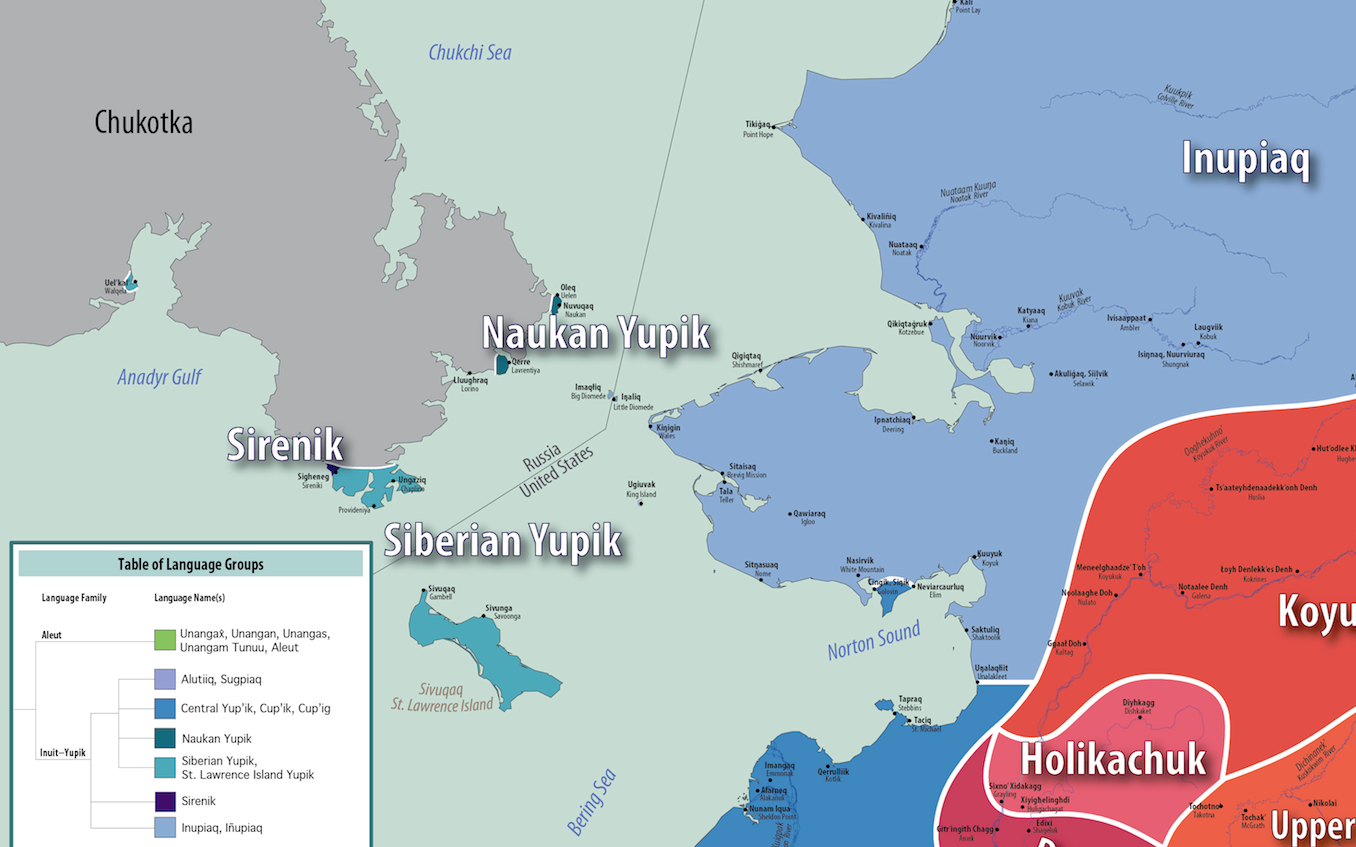
\includegraphics[scale=0.68]{anla-map.png}
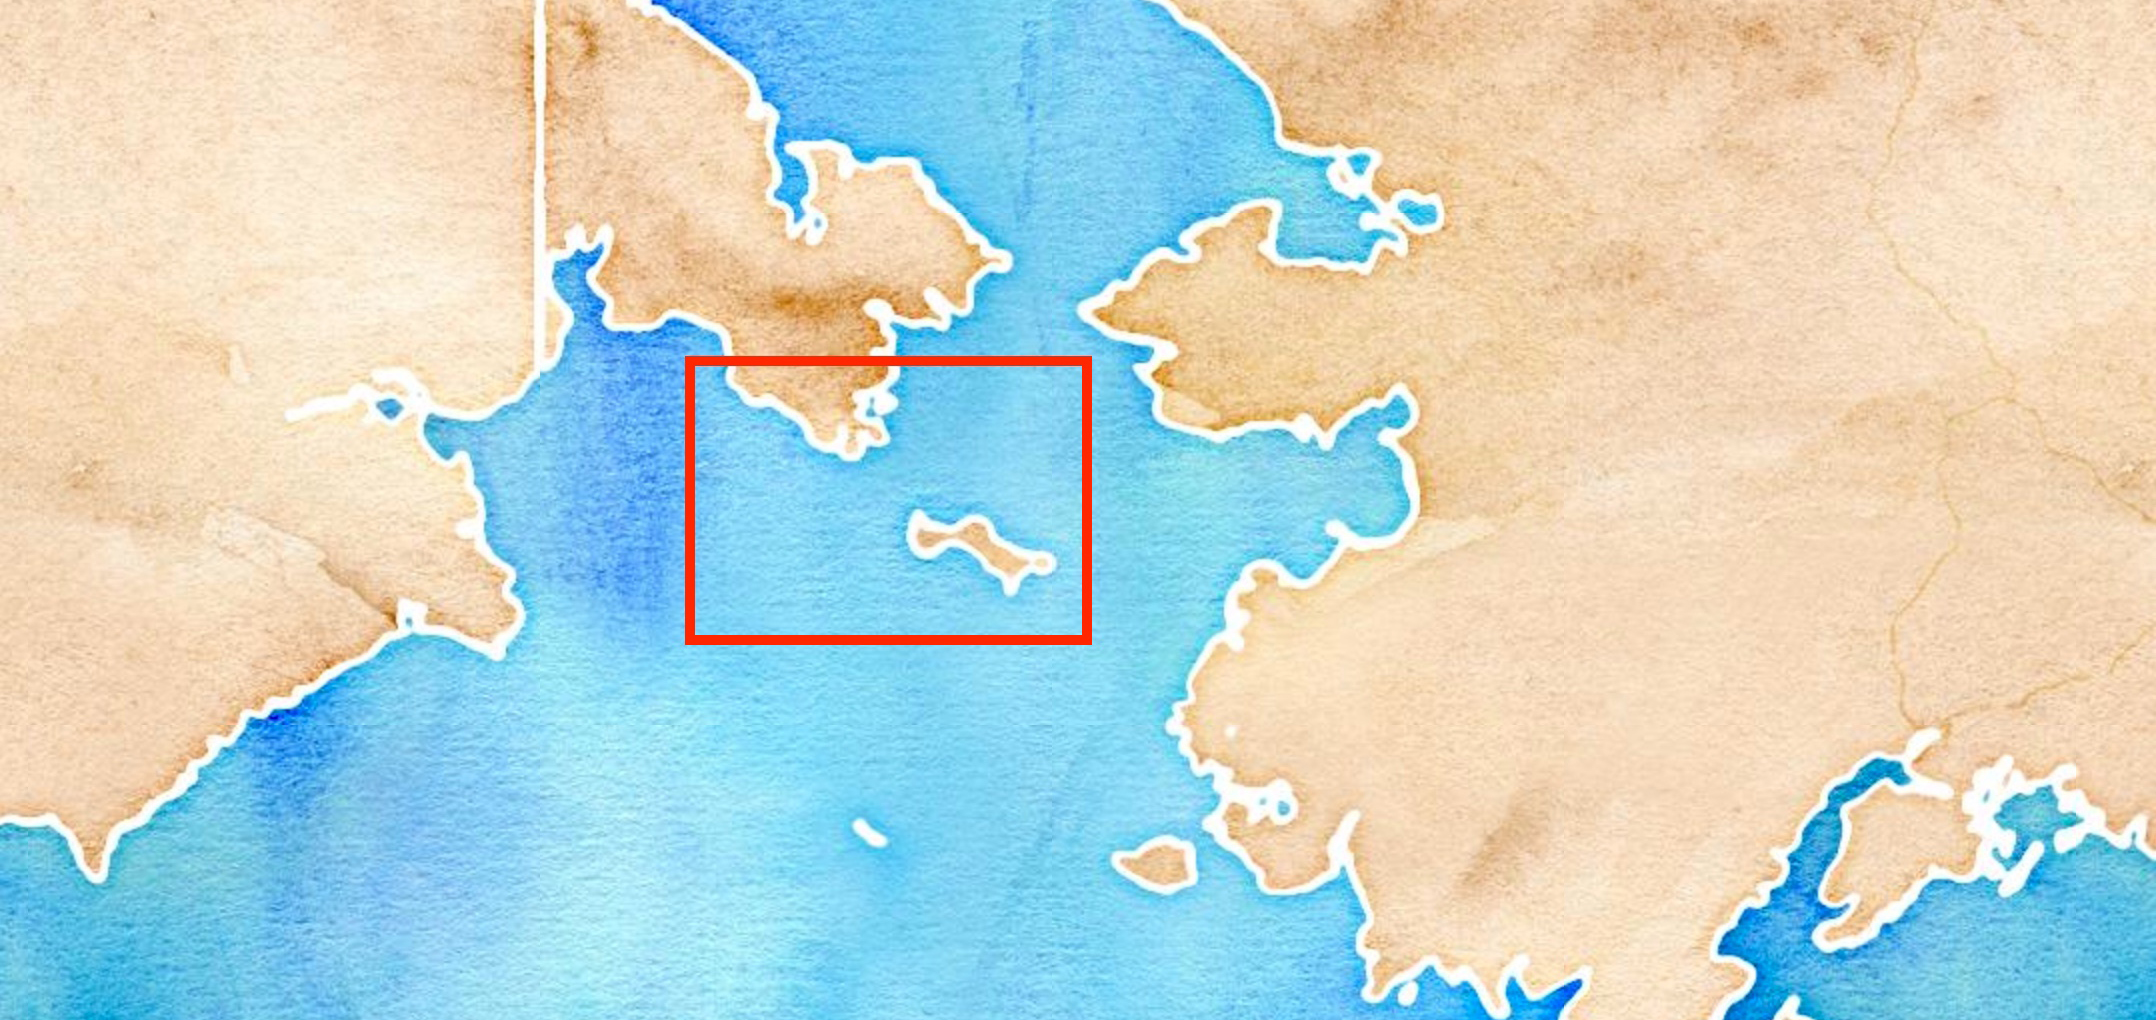
\includegraphics[scale=0.68]{map-box.jpg}
\end{minipage}%
\begin{minipage}{0.3\textwidth}
 \begin{tikzpicture}
    \begin{axis}[
        ybar stacked,
        cycle list name=exotic,
    	bar width=20pt,
    	nodes near coords,
    	height=7cm,
    	width=10cm,
        %enlargelimits=0.15,
        legend style={at={(0.5,-1)},
          anchor=north,legend columns=-1},
        %ylabel={\#participants},
        yticklabels={,,},
        symbolic x coords={SLI, Chukotka, Mainland AK},
        xtick=data,
        x tick label style={rotate=45,anchor=east},
        ]
    \addplot+[ybar, fill=teal!40] plot coordinates {(SLI, 1000) (Chukotka, 200) (Mainland AK, 200)};
    \addplot+[ybar, fill=orange!30] plot coordinates {(SLI, 300) (Chukotka, 1000) (Mainland AK, 200)};
    \legend{\strut L1 Speakers, \strut Population}
    \end{axis}
    \end{tikzpicture}
\end{minipage}
\end{figure}
\end{comment}

\begin{center}
\begin{tikzpicture}[scale=2.25, every node/.style={transform shape}, point/.style={rectangle,draw,fill=black,inner sep=0pt,minimum size=0.001mm},]
%\node (IYA) [] {Inuit-Yupik-Aleut};
%\node (IY) [] {Inuit-Yupik};
%\node (A) [] {Aleut};

\node[point] (root) []                  {};
\node[point] (IYA)  [right=35mm of root] {};
%
\node[point] (A)    [below=28mm of IYA]  {};
\node[point] (IY1)  [above=14mm of IYA]  {};
%
\node[point] (IY2)  [right=10mm of IY1]  {};
\node[point] (I)    [above=6mm of IY2]  {};
\node[point] (S)    [below=10mm of I]    {};
\node[point] (Y)    [below=16mm of S]    {};
\node[point] (Y0)   [right=20mm of Y]    {};
\node[point] (Y1)   [above=9mm of Y0]    {};
\node[point] (Y2)   [below=6mm of Y1]    {};
\node[point] (Y3)   [below=6mm of Y2]    {};
\node[point] (Y4)   [below=6mm of Y3]    {};
\node[point] (Y5)   [above=6mm of Y1]    {};

\node[] (Aleut)  [right=13.5mm of A]  {\tiny Unangam Tunuu (Aleut)};
\node[] (Inuit)  [right=3mm of I]  {\tiny Inuit};
\node[] (Sirenik)  [right=27.1mm of S]  {\tiny Sirenik};
\node[] (Siberian) [right=7mm of Y1] {\tiny \textbf{St. Lawrence Island Yupik}};
\node[] (Naukan) [right=7mm of Y2] {\tiny Naukan};
\node[] (Alaskan) [right=7mm of Y3] {\tiny Central Alaskan Yup'ik};
\node[] (Alutiiq) [right=7mm of Y4] {\tiny Alutiiq / Sugpiaq};

%\draw (root) node[below]{Inuit-Yupik-Aleut} -- (IYA);
\draw (root) -- (IYA) node [midway, above] {\tiny Inuit-Yupik-} node [midway, below] {\tiny \hspace{-1cm} Unangam Tunuu};
\draw (A)  -- (IY1);
\draw (IY1) -- (IY2);
\draw (A) -- (Aleut);
\draw (I) -- (Y);
\draw (I) -- (Inuit);
\draw (S) -- (Sirenik);
\draw (Y) -- (Y0) node [midway, below] {\tiny Yupik};
\draw (Y1) -- (Y4);
\draw (Y1) -- (Siberian);
\draw (Y2) -- (Naukan);
\draw (Y3) -- (Alaskan);
\draw (Y4) -- (Alutiiq);
\draw[dotted] (Y1) -- (Y5);

\end{tikzpicture}
\end{center}

\end{block}
\end{column}
\end{columns}

%%%%%% END ROW %%%%%%

\vspace{28pt}


\begin{columns}[T]
\begin{column}{0.3\textwidth}
\begin{block}{Digitize Legacy Resources}
Numerous Yupik-language texts were developed in the Soviet Union in the early 20th century and in Alaska in the mid- to late-20th century.
%
One project goal is the digitization of these texts.
%
To date, we have digitized \citet{Apassingok:LoreSLI, Apassingok:Readers} and \citet{Koonooka:2003}.
%
%The most notable of the Latin-orthography texts include the three-volume \textit{Lore of St.\ Lawrence Island} collection \citep[][stories in Yupik together with free translations into English]{Apassingok:LoreSLI}, a sequence of elementary readers \citep{Apassingok:Readers}, and a collection of Chukotkan Yupik oral narratives \citep{Koonooka:2003}.

\end{block}

\begin{block}{Yupik Grammar Overview}

 \begin{itemize}
 \setlength\itemsep{18pt}
    \item Polysynthetic
    \item Ergative-absolutive
    \item 4 persons, 3 numbers
    \item Fairly free word order
    \item $\sim$500 particles
    \item Extensive system of demonstratives
    \item $\sim$600+ derivational suffixes
     \item General structure (inflected verb):
    %\begin{itemize}
        %\item 6000+ \textit{Noun} and \textit{Verb} roots
        %\item 600+ Derivational Suffixes
        %\item 2000+ Inflectional Suffixes
        %\item 11 Enclitics
    %\end{itemize}
    
    \vspace{24pt}
    
    \hspace*{-42pt}
    \begin{tikzpicture}
    \tikzstyle{rec} = [rectangle, rounded corners,draw,fill=orange!30]
    \node [rec] {Root};
    \node [xshift=2cm] {+};
    \node [rec, xshift=5.5cm] {Derivation};
    \node [xshift=9cm] (plus1) {+};
    \node [rec, xshift=11cm] {NEG};
    \node [xshift=13cm] {+};
    \node [rec, xshift=15.6cm] {TMMA};
    \node [xshift=18.2cm] {+};
    \node [rec, xshift=19.9cm] {Infl};
    \node [xshift=21.6cm] (plus1) {+};
    \node [rec, xshift=23.5cm] (is) {Encl};
    \end{tikzpicture}
    
    \vspace{18pt}
\end{itemize}
\vspace*{9mm}
\end{block}
\end{column}

\begin{column}{0.3\textwidth}
\begin{block}{Language Documentation \& Analysis}
%
A major goal of our fieldwork is the documentation of Yupik phonology, morphology, and syntax beyond that described by \citet{Krauss:1975} \& \citet{Jacobson:2001}.
%
We hope this will be of use for developing modern pedagogical materials for Yupik language instruction and immersion programs.
%Another major goal is the development of modern pedagogical materials for Yupik language instruction and language immersion programs.

\end{block}

%
\begin{minipage}{0.49\textwidth}
%\begin{center}
\hspace*{-7mm}
\renewcommand{\arraystretch}{0.75}
\begin{tabular}{r|r|r|}
\cline{2-3}
 & \scriptsize L1 Yupik & \scriptsize Yupik \\ 
 & \scriptsize Speakers & \scriptsize Population \\ \hline
\multicolumn{}{|r|}{\scriptsize Mainland Russia}  &  \scriptsize $<$200 & \scriptsize 800      \\
\multicolumn{}{|r|}{\scriptsize St.~Lawrence Island} & \scriptsize 500---700 & \scriptsize 1300      \\
\multicolumn{}{|r|}{\scriptsize Mainland Alaska}    & \scriptsize  $<$200 & \scriptsize  400      \\
\hline
\hline
\multicolumn{}{|c|}{\scriptsize Total} & \scriptsize 800---900 & \scriptsize 2400---2500 \\ \hline
\end{tabular}
%    \end{center}
\end{minipage}
%
\begin{minipage}{0.49\textwidth}
\hspace*{8.5mm}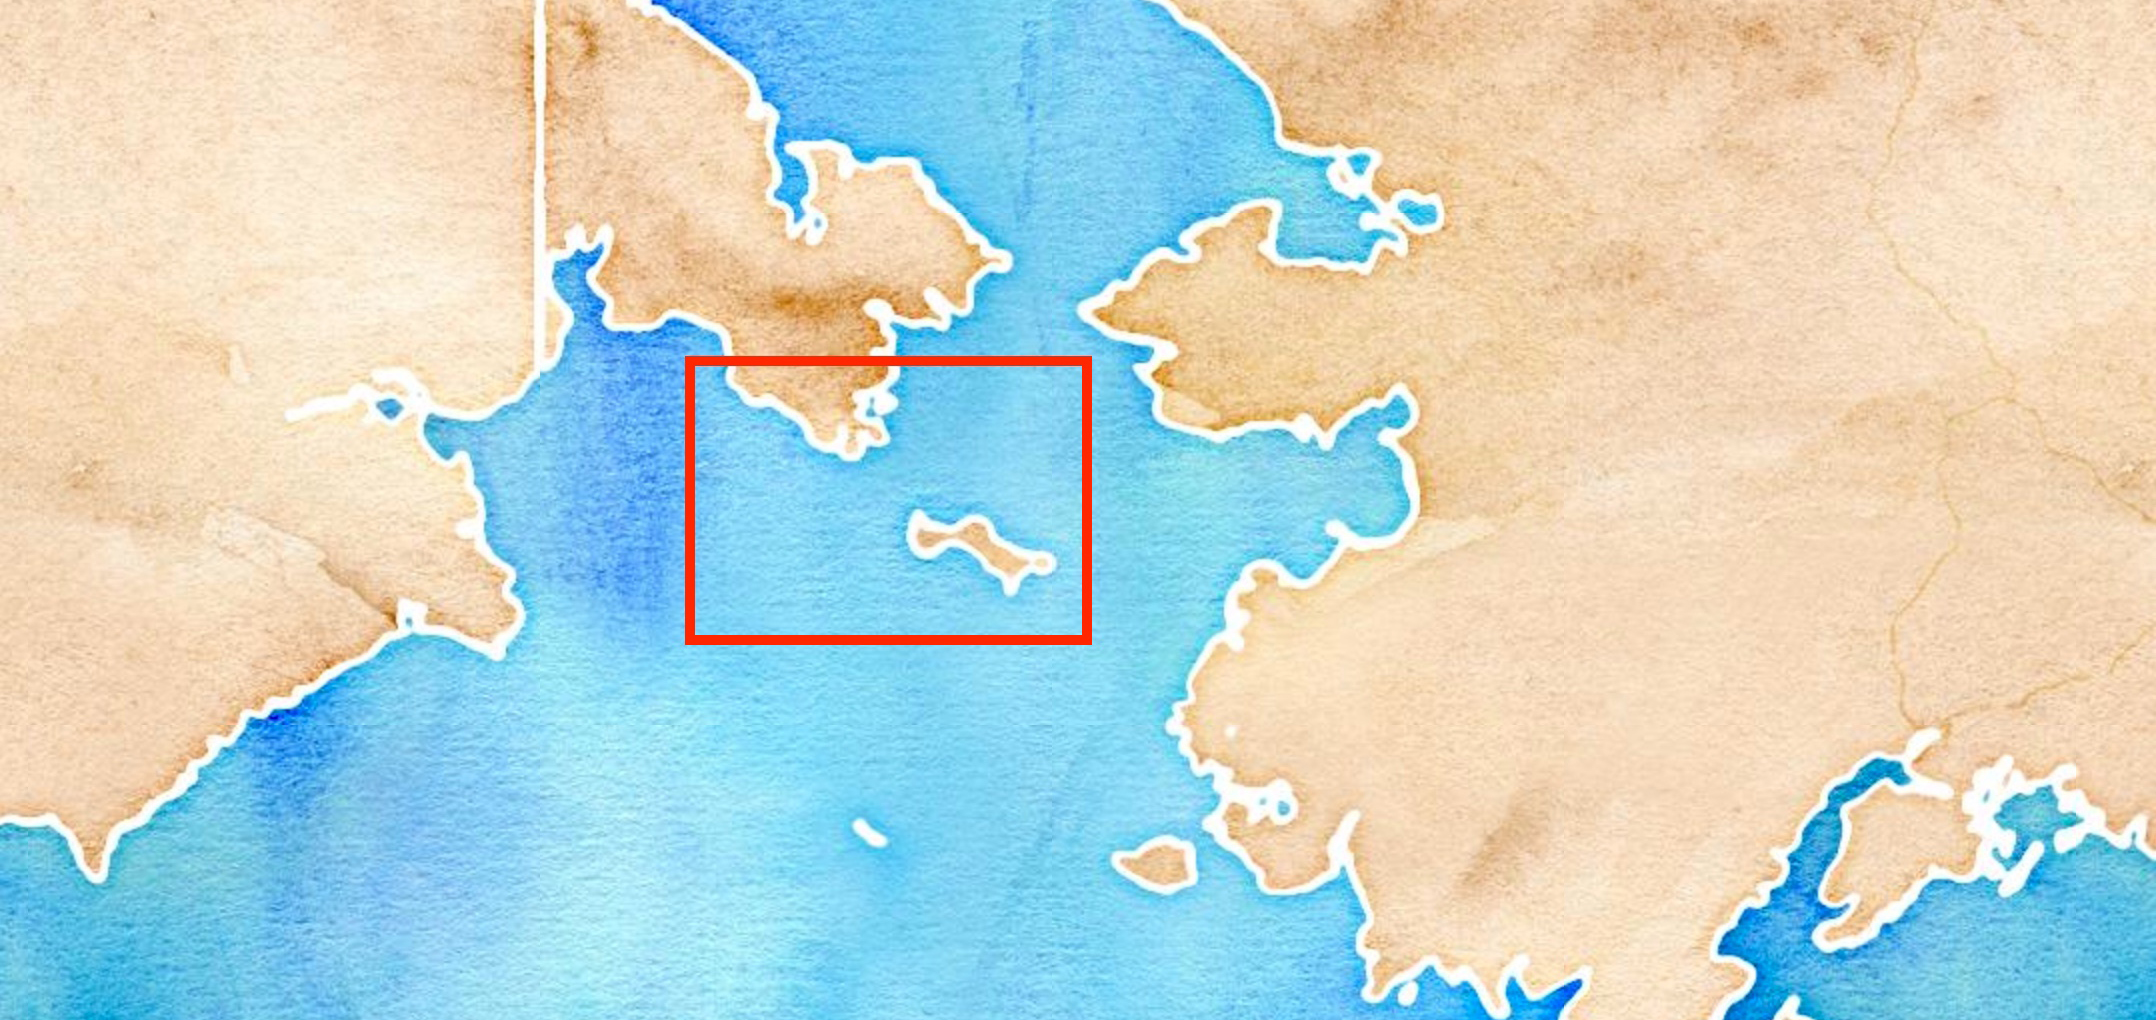
\includegraphics[scale=0.34]{map-box.jpg}
%
\includegraphics[width=\textwidth]{map-box2.jpg}
\end{minipage}%
\vspace{18pt}

\begin{block}{Fieldwork on St.~Lawrence Island}

\begin{itemize}
 \setlength\itemsep{18pt}
        \item Semi-naturalistic production
        
        \item Targeted elicitation of morphosyntactic / semantic phenomena and analyzer errors
        
        \item Detailed positional and semantic work with derivational morphology
        
        \item Translation of Yupik texts into English
        
        \item Expansion of current lexicon

    \end{itemize}
    \vspace*{3mm}
\end{block}

\end{column}

\begin{column}{0.29\textwidth}
\begin{block}{Computational Tool Development}
%
We view computational tool development as integral to language documentation and revitalization.
%
%To date, we have developed a web-based basic spell-checker \& transliterator, a finite-state morphological analyzer, a basic neural morphological analyzer, \& electronic  dictionary.
%
To date, we have developed a suite of web-based orthographic utilities \citep{SchwartzChen:2017}, a finite-state morphological analyzer \citep{ChenSchwartz:LREC:2018}, a preliminary neural morphological analyzer \citep{Schwartz:etal:ComputEL:2019}, and an electronic  dictionary \citep{Hunt:etal:ICLDC:2019}.
%
\end{block}

\begin{block}{Morphological Analysis in the Field}

\begin{itemize}
%    \item Finite-state morphological analyzer implemented in \texttt{foma} \citep{Hulden:2009} 
    \item Finite-state analyzer implements Yupik grammar of \citet{Jacobson:2001} using \texttt{foma} \citep{Hulden:2009} 

%\begin{comment}
\vspace{18pt}

\item User provides Yupik surface form. \\ Potential morphological analyses are returned:

\vspace{9pt}

\fbox{
\begin{minipage}{19.5em}
    {\ttfamily \footnotesize
        apply up$\textrangle$ \textbf{mangteghaghllagek} \\
        \textrm{\textbf{\textit{mangteghagh--ghllag[N$\rightarrow$N][N][Abs][Unpd][Du]}}} \\
        \textrm{\textbf{\textit{mangteghagh--ghllag[N$\rightarrow$N][N][Rel][Unpd][Du]}}}
    }
\end{minipage}
}

\vspace{24pt}

\item User provides Yupik underlying form. \\ Corresponding Yupik surface form is returned:

\vspace{9pt}

\fbox{
\begin{minipage}{19.5em}
    {\ttfamily \footnotesize
        apply down$\textrangle$ \textrm{\textbf{\textit{mangteghagh--ghllag[N$\rightarrow$N][N][Abs][Unpd][Du]}}} \\
        \textbf{mangteghaghllagek}
    }
\end{minipage}
}

\end{itemize}
\begin{comment}
\fbox{
\begin{minipage}{20em}
    {\ttfamily \footnotesize
        foma[0]: load ess.fomabin \\
        3.0 MB.  60980 states, 194963 arcs, Cyclic. \\
        foma[1]: apply up \\
        apply up$\textrangle$ \textbf{mangteghaghllagek} \\
        \textrm{\textbf{\textit{mangteghagh--ghllag[N$\rightarrow$N][N][Abs][Unpd][Du]}}} \\
        mangteghagh--ghllag[N$\rightarrow$N][N][Rel][Unpd][Du] \\
        foma[1]: apply down \\
        apply down$\textrangle$ mangteghagh--ghllag[N$\rightarrow$N][N]
        [Abs][Unpd][Du] \\
        mangteghaghllagek
    }
\end{minipage}
}
\end{comment}
%\end{comment}
\end{block}
\end{column}
\end{columns}

\begin{comment}
%%%%%% START ROW %%%%%%
\begin{columns}

% Project Components %
\begin{column}{0.95\textwidth}
\begin{block}{Project Components}
\begin{columns}



\begin{column}{0.3\columnwidth}

\begin{itemize}
    \item \textbf{Digitize Legacy Resources}
    \vspace{18pt}
    \begin{itemize}

    
    \setlength\itemsep{18pt}
        \item Ethnographies / folk stories / fieldwork papers
        \item Bilingual-bicultural pedagogical materials
        
        \item OBJECTIVES:
        \vspace{12pt}
        \begin{itemize}
        \setlength\itemsep{12pt}
            \item Increase access for community
            \item Build corpus of Yupik texts
        \end{itemize}
    \end{itemize}
\end{itemize}
\end{column}

\begin{column}{0.3\columnwidth}
\begin{itemize}
    \item \textbf{Computational Resources}
    \vspace{18pt}
    \begin{itemize}
    \setlength\itemsep{5pt}
        \item Web-based orthographic utilities \\ \citep{SchwartzChen:2017}
        \item Finite-state morphological analyzer \\ \citep{ChenSchwartz:LREC:2018}
        \item Preliminary neural morphological analyzer \\ \citep{Schwartz:etal:ComputEL:2019}
        \item Electronic Yupik-English dictionary \\ \citep{Hunt:etal:ICLDC:2019}
    \end{itemize}
\end{itemize}
\end{column}

\begin{column}{0.3\columnwidth}
\begin{itemize}
    \item \textbf{Documentation/Analysis}
    \vspace{18pt}
    \begin{itemize}
    \setlength\itemsep{18pt}
        \item Un(der)documented linguistic phenomena
        \item Clarify conflicting information in existing literature
        
        \item OBJECTIVES:
        \vspace{12pt}
        \begin{itemize}
        \setlength\itemsep{12pt}
            \item More thorough documentation of Yupik
            \item Better documentation for developing modern pedagogical materials and desired technology
        \end{itemize}
    \end{itemize}
\end{itemize}
\end{column}

\end{columns}
\end{block}
\end{column}

\end{columns}
%%%%%% END ROW %%%%%%
\end{comment}

\vspace{28pt}



%\vspace{28pt}

{\LARGE \textcolor{orange}{\textbf{\PencilLeftDown}} \textcolor{teal}{Processes and Insights from the Field: Establishing the \textit{Virtuous Cycle} - - - - - - - - - - - - - - - - - - -}}

\vspace{28pt}

%%%%%% START ROW %%%%%%
\begin{columns}

% Scenario 1 %
\begin{column}{0.3\textwidth}
\begin{block}{The Virtuous Cycle}
\vspace*{8mm}
\begin{itemize}
\setlength\itemsep{48pt}
    \item \textbf{SCENARIO 1}: Analyzer fails to analyze a word or produce the known correct analysis
    \vspace{24pt}
    \begin{itemize}
    \setlength\itemsep{24pt}
    \item \textit{Hypothesis}: Word may involve linguistic phenomena that are currently undocumented or not well-documented
            
    \item \textit{Solution}: Inquire about the word with a speaker; % to gain insight into its morphological analysis; 
    adjust analyzer or lexicon as appropriate
   

        
    \end{itemize}
  
    \item
    \begin{tabular}[t]{c}
    Fieldwork Elicitation \\
    $\downarrow$ \\
    Larger Corpus \\
    $\downarrow$ \\\
    More Accurate Morphological Analyzer
    \end{tabular}
\end{itemize}
\vspace*{8mm}
\end{block}
\end{column}

% Virtuous Cycle Image %
\begin{column}{0.3\textwidth}
\hspace*{24pt}
\begin{tikzpicture}[scale=6, xscale=1.22, yscale=0.35]
\draw[fill=orange!40, draw=orange!40, line width=1pt, rotate=-170] (0:1.4cm) arc (0:-180:1.4cm) -- (-180:1.76cm) -- (-1.25,.5) -- (-180:.75cm) -- (-180:1.1cm) arc (-180:0:1.1cm)--cycle;
\end{tikzpicture}

\begin{tikzpicture}
\node [text width=6cm, text centered] at (-1.75, -0.25) {More Guided \\ Fieldwork};
\node [text width=7cm, text centered] at (7.5, -0.25) {\textbf{\large THE \\ VIRTUOUS CYCLE}};
\node [text width=7cm, text centered] at (17, -0.25) {More Accurate \\ Analyzer};
\end{tikzpicture}

\begin{tikzpicture}[scale=6, xscale=1.22, yscale=0.35]
\draw[fill=orange!40, draw=orange!40, line width=1pt, rotate=10] (0:1.4cm) arc (0:-180:1.4cm) -- (-180:1.76cm) -- (-1.25,.5) -- (-180:.75cm) -- (-180:1.1cm) arc (-180:0:1.1cm)--cycle;
\end{tikzpicture}

\begin{block}{Examples}
\small
        \begin{itemize}
            \item \textit{aatqus}, \textit{aghnas}, \textit{akughvigaas}, etc. \\ Previously undocumented phonological (and orthographic) process applying across word boundaries: 
            word-final /t/ $\rightarrow$ /s/ when followed by word-initial /t/ %(lenition: word-final /t,k,q/ become corresponding fricatives when followed by identical sound)
            
            \item \textit{allgeqestaamaan} - Previously undocumented derivational suffix, \textit{-kestamaan} (``in the time of'')
        \end{itemize}
\end{block}
\end{column}

% Scenario 2 %
\begin{column}{0.3\textwidth}
\begin{block}{The Virtuous Cycle ({\small CONT})}
\vspace*{8mm}
\begin{itemize}
\setlength\itemsep{48pt}
    \item \textbf{SCENARIO 2}: Elicitor successfully analyzes a word with the analyzer
    \vspace{24pt}
    \begin{itemize}
    \setlength\itemsep{24pt}
    \item \textit{Result 1}: One Analysis $\rightarrow$ Follow-up with speaker to confirm correctness
            
    \item \textit{Result 2}: Multiple Analyses $\rightarrow$ Follow-up with speaker to determine the correct analysis
    \end{itemize}
    
    \item
    \begin{tabular}[t]{c}
    More Accurate Morphological Analyzer \\
    $\downarrow$ \\
    More Efficient Analysis of New Data \\
    $\downarrow$ \\\
    More Guided Future Elicitations
    \end{tabular}
\end{itemize}
\vspace*{8mm}
\end{block}
\end{column}

\end{columns}
%%%%%% END ROW %%%%%%

\vspace{18pt}

%%%%%% START ROW %%%%%%
\begin{columns}[T]

% Implications %
\begin{column}{0.46\textwidth}
\begin{block}{Implications}

\begin{itemize}
    \item The \textit{virtuous cycle} benefits all sides of the research process:
        \vspace{18pt}
        \begin{itemize}
        \setlength\itemsep{18pt}
        
            \item \textbf{Computational Linguistics}
            \vspace{12pt}
            \begin{itemize}
            \setlength\itemsep{12pt}
                \item Analyzer is improved more quickly and more accurately
            
                \item Analyzer facilitates development of computational resources for the community
            \end{itemize}
        
             \item \textbf{Language Documentation}
            \vspace{12pt}
            \begin{itemize}
            \setlength\itemsep{12pt}
                \item Elicitation/documentation is expedited with a better-performing analyzer
            
                \item Documentation is improved as the analyzer identifies gaps in existing descriptions
            \end{itemize}
                
            \item \textbf{Related Languages}
            \vspace{12pt}
            \begin{itemize}
            \setlength\itemsep{18pt}
                \item Other languages in the family may benefit from the improved documentation of Yupik
                
                \item Other underdocumented, polysynthetic languages may benefit by applying the \textit{virtuous cycle}
            \end{itemize}
    \end{itemize}
\end{itemize}
\vspace*{12mm}
\end{block}
\end{column}

\begin{column}{0.46\textwidth}
\begin{block}{References}
\tiny
\nocite{*}
\bibliography{main}
%\bibliographystyle{acl_natbib_nourl}
\bibliographystyle{plainnat}
\end{block}
\begin{block}{Acknowledgements}
\tiny
Portions of this work were funded by NSF Documenting Endangered Languages Grants \#BCS 1761680 and 1760977, a University of Illinois Graduate College \textit{Illinois Distinguished Fellowship}, a George Mason University Mathy Junior Faculty Award in the Arts and Humanities, and George Mason University Presidential Scholarship. Special thanks to the Yupik speakers who have shared their language and culture with us.
\end{block}
\end{column}

\end{columns}
%%%%%% END ROW %%%%%%

\end{frame}
\end{document}